
\documentclass[submit]{harvardml}

% You don't need to change these.
\course{CS181-S19}
\assignment{Assignment \#3}
\duedate{11:59pm March 29, 2019}

\usepackage[OT1]{fontenc}
\usepackage[colorlinks,citecolor=blue,urlcolor=blue]{hyperref}
\usepackage[pdftex]{graphicx}
\usepackage{subfig}
\usepackage{fullpage}
\usepackage{amsmath}
\usepackage{amssymb}
\usepackage{color}
\usepackage{todonotes}
\usepackage{listings}
\usepackage{common}
\usepackage{bm}

\usepackage[mmddyyyy,hhmmss]{datetime}

\definecolor{verbgray}{gray}{0.9}

\lstnewenvironment{csv}{%
  \lstset{backgroundcolor=\color{verbgray},
  frame=single,
  framerule=0pt,
  basicstyle=\ttfamily,
  columns=fullflexible}}{}

\begin{document}
\begin{center}
{\Large Homework 3: Max-Margin, Ethics, Clustering}\\
\end{center}
\subsection*{Introduction}

This homework assignment will have you work with max-margin methods
and clustering, as well as an ethics assignment.  The aim of the
assignment is (1) to further develop your geometrical intuition behind
margin-based classification and decision boundaries, (2) try coding a
simple K-means classifier, and (3) to have you reflect on the ethics
lecture and to address the scenario discussed in class in more depth
by considering the labor market dynamically.

We encourage you to first read the Bishop textbook coverage of these topics,
particularly: Section 7.1 (Max-Margin and SVMs) and Section 9.1 (Clustering).
Chapters 5 and 6 of the student textbook are also relevant.

There is a mathematical component and a programming component to this
homework.  Please submit your PDF, tex, and Python files to Canvas,
and push all of your work to your GitHub repository. If a question
requires you to make any plots, like Problem 2, please include those
in the writeup.

\newpage
%%%%%%%%%%%%%%%%%%%%%%%%%%%%%%%%%%%%%%%%%%%%%
% Problem 1
%%%%%%%%%%%%%%%%%%%%%%%%%%%%%%%%%%%%%%%%%%%%%
\begin{problem}[Fitting an SVM by hand, 7pts]
  For this problem you will solve an SVM without the help of a
  computer, relying instead on principled rules and properties of
  these classifiers.

Consider a dataset with the following 7 data points each with $x \in \reals$ : \[\{(x_i, y_i)\}_i =\{(-3 , +1) , (-2 , +1 ) , (-1,  -1 ), (0, +1), ( 1 , -1 ), ( 2 , +1 ) , ( 3 , +1 )\}\] Consider
mapping these points to $2$ dimensions using the feature vector $\bphi(x) =  (x, -\frac{8}{3}x^2 + \frac{2}{3}x^4 )$. The hard margin classifier training problem is:
%
\begin{align*}
  &\min_{\mathbf{w}, w_0} \|\mathbf{w}\|_2^2 \label{eq:dcp} \\
  \quad \text{s.t.} \quad & y_i(\mathbf{w}^\top \bphi(x_i) + w_0) \geq 1,~\forall i \in \{1,\ldots, n\}\notag
\end{align*}

The exercise has been broken down into a series of questions, each
providing a part of the solution. Make sure to follow the logical structure of
the exercise when composing your answer and to justify each step.

\begin{enumerate}
\item Plot the transformed training data in $\reals^2$ and draw the decision boundary
of the max margin classifer.
%
\item  What is the value of the margin achieved by the optimal
decision boundary? 
%
\item What is a vector that is orthogonal to the decision boundary?

%
\item Considering discriminant $h(\bphi(x);\boldw,w_0)=\boldw^\top\bphi(x) +w_0$, 
give an expression for {\em all possible} $(\boldw,w_0)$ that define
the optimal decision boundary. Justify your answer.

  \item Consider now the training problem. Using your answers so far,
    what particular solution to $\boldw$ will be optimal for this
    optimization problem?

  \item Now solve for the corresponding value of $w_0$, using your
    general expression from part~(4.) for the optimal decision
    boundary.  Write down the discriminant function
    $h(\bphi(x);\boldw,w_0)$.


\item What are the support vectors of the classifier?  Confirm that
  the solution in part~(6.) makes the constraints above binding for
  support vectors.

\end{enumerate}

\end{problem}
\subsection*{Solution}

\begin{enumerate}
    \item The transformed data looks like
    
    \begin{center}
        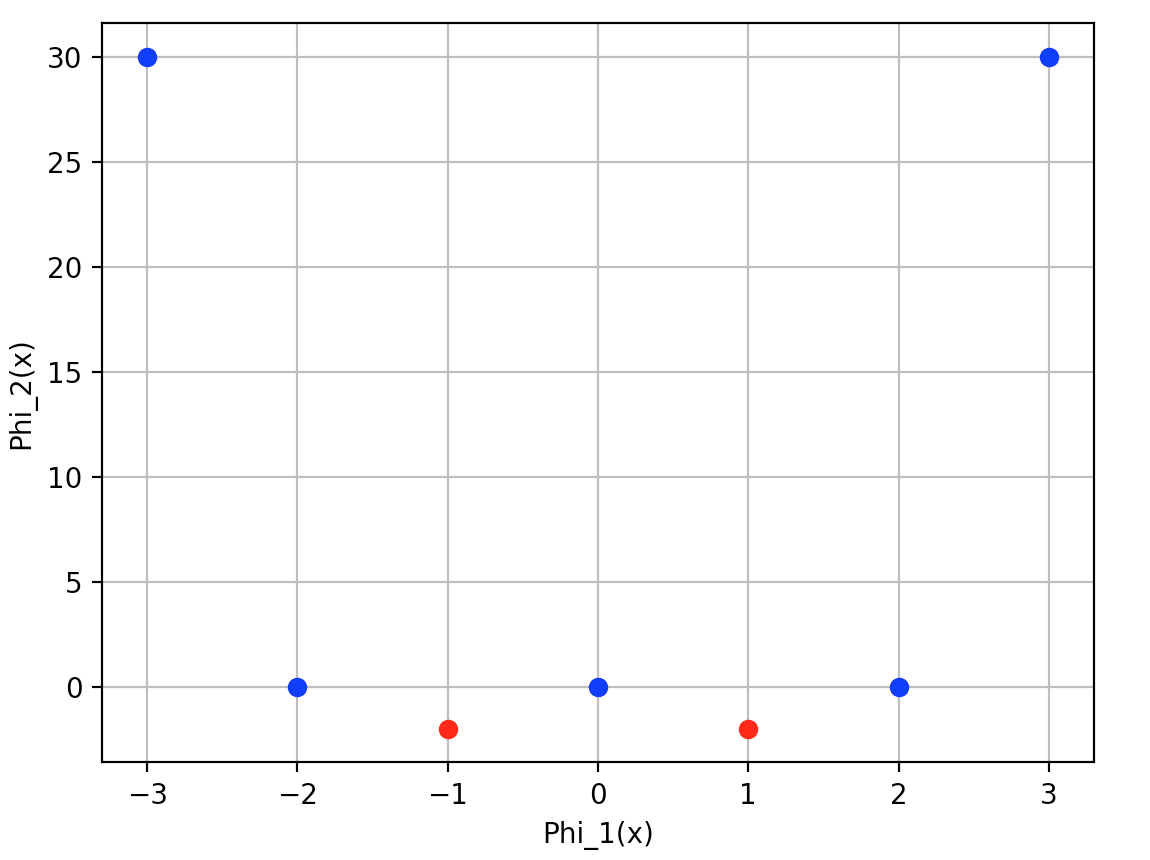
\includegraphics[scale=0.5]{1_11.png}
    \end{center}
    
    where blue points correspond to $y = +1$ and red points correspond to $y=-1$. By inspection, we see that the max-margin decision boundary will be at $\phi_2(x) = -1$. Including this, the plot is
    
    \begin{center}
        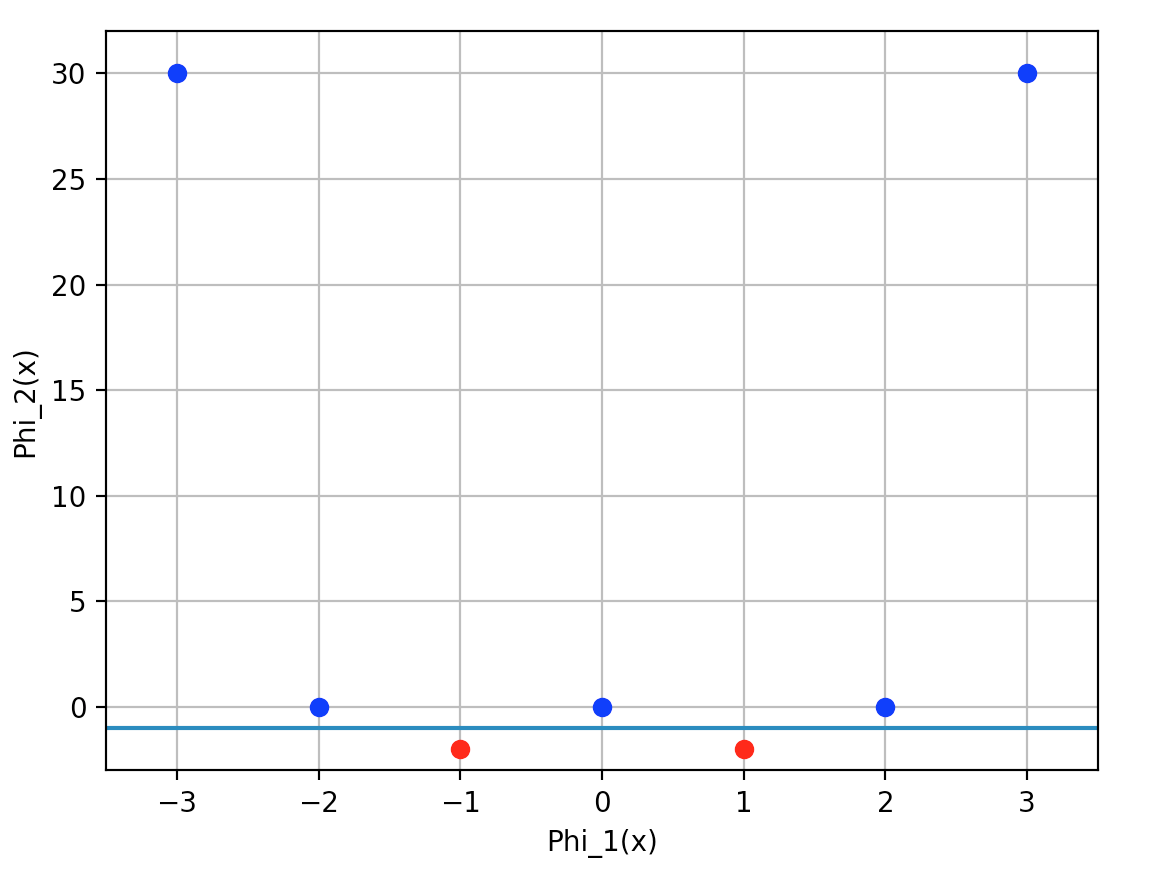
\includegraphics[scale=0.5]{1_1.png}
    \end{center}
    
    \item By inspection, the optimal decision boundary achieves a margin of $\boxed{1}$.
    
    \item We see that a vertical line in the $[\phi_1(x), \phi_2(x)]$ space will be perpendicular to the decision boundary. Hence, $\boxed{[0,1]^T}$ is orthogonal to the decision boundary.
    
    \item Since $[0,1]^T$ is orthogonal to the decision boundary, it is a valid choice for \textbf{w}. Plugging this into our discriminant, which is 0 at the boundary, we have
    
    $$ h(\bphi(x);\boldw,w_0)= 0 = [0,1]\bphi(x) +w_0 = [0,1] [\phi_1(x), \phi_2(x)] +w_0 $$ 
    
    Now, since we determined that $\phi_2(x) = -1$ is our boundary, this becomes
    
    $$ = [0,1] [\phi_1(x), -1] +w_0 = w_0 - 1 = 0$$ 
    
    and we conclude that $(\boldw = [0,1]^T,w_0 = 1)$ is a valid $(\boldw,w_0)$ combination. However, notice that the discriminant equation is invariant to scaling at the boundary since it is equal to $0$. In other words, $\bold{w'} = c\boldw, w_0' = cw_0$ are also valid weights for this problem because $c[0,1][\phi_1(x), -1] +cw_0 = cw_0 - c = 0$ implies that if $\boldw = [0,c]^T$ then as long as $w_0 = c$ our boundary condition will still work. Hence, we realize that we can multiply the boundary condtion by $c$ and get that in general any $(\boldw,w_0)$ must have the form $\boxed{(\boldw = [0,c]^T,w_0 = c)}$.
    
    \item Now that we are considering the training problem, we must use actual data from our dataset. Specifically, we know that we are minimizing the norm of $\boldw$ subject to $y_i(\mathbf{w}^\top \bphi(x_i) + w_0) \geq 1$. This will hold with equality for our support vectors, the points closest to the boundary. Hence, we can plug in one of these points (transformed into the $\bold\phi$ space) and solve for the appropriate $(\boldw,w_0)$ for this problem. Let's use the point (-2,0) which has class $+1$. Using the general $(\boldw,w_0)$ we found earlier, we have
    
    $$ +1([0,c][-2,0]^T + c) = 1 \implies c = 1$$
    
    Hence, we have that  $\boxed{(\boldw = [0,1]^T,w_0 = 1)}$ will be the optimal solution for this optimization problem. 
    
    Alternatively, we could have used that $\|\mathbf{w}\|_2^2 = 1$ in the hard boundary optimization problem. So, $\|[0,c]^T\|_2^2 = 1$ and we see that $\mathbf{w} = [0,1]^T$ for this to be true.
    
    \item See the previous part. We have that $\boxed{w_0 = 1}$. This agrees with my general expression from part 4. The discriminant function is thus
    
    $$\boxed{h(\bphi(x);\boldw,w_0)= [0,1] \bphi(x) + 1 }$$ 
    
    \item By inspection, there are five support vectors. For the $y = +1$ class, these are (-2,0), (0,0), and (2,0). For the $y = -1$ class, these are (-1,-2) and (1,-2). I have given all of these in the transformed $\bold\phi$ space. Indeed, as shown below, the constraint is binding for these support vectors.
    
    $$ (-2,0): +1([0,1][-2,0]^T + 1) = 1$$
    $$ (0,0): +1([0,1][0,0]^T + 1) = 1$$
    $$ (2,0): +1([0,1][2,0]^T + 1) = 1$$
    $$ (-1,-2): -1([0,1][-1,-2]^T + 1) = 1$$
    $$ (1,-2): -1([0,1][1,-2]^T + 1) = 1$$
    
    The untransformed points which correspond to these support vectors are, respectively, are $$(-2,+1),  (0,+1), (2,+1), (-1,-1), (1,-1) $$.
    
\end{enumerate}

\newpage
%%%%%%%%%%%%%%%%%%%%%%%%%%%%%%%%%%%%%%%%%%%%%
% Problem 2
%%%%%%%%%%%%%%%%%%%%%%%%%%%%%%%%%%%%%%%%%%%%%

\begin{problem}[K-Means, 10pts]

For this problem you will implement K-Means clustering from
scratch. Using \texttt{numpy} is fine, but don't use a third-party
machine learning implementation like \texttt{scikit-learn}. You will
then apply this approach to clustering of image data.

We have provided you with the MNIST dataset, a collection of
handwritten digits used as a benchmark of image recogntion (you can
learn more about the data set at
\url{http://yann.lecun.com/exdb/mnist/}). The MNIST task is widely
used in supervised learning, and modern algorithms with neural
networks do very well on this task.

Here we will apply unsupervised learning to MNIST. You have been given
representations of 6000 MNIST images, each of which are $28\times28$
greyscale handwritten digits. Your job is to implement K-means
clustering on MNIST, and to test whether this relatively simple
algorithm can cluster similar-looking images together.

The given code loads the images into your environment as a 6000x28x28
array.  In your code, you may use the $\ell_2$ norm as your distance
metric. (You should feel free to explore other metrics than the
$\ell_2$ norm, but this is strictly optional.)

\begin{itemize}

\item Starting at a random initialization and some choice of K, plot
  the K-means objective function as a function of iteration and verify
  that it never increases.

\item Run the K-means algorithm from several different restarts for
  different values of K.  Plot the final K-means objective as a
  function of K with errorbars over the random restarts.  How does the
  objective and the variance of the objective change with K?  
  
\item For $K=10$, for a couple of random restarts, show the mean
  images for each cluster.  To render an image, use the pyplot
  \texttt{imshow} function.

\item Now, before running K-means, standardize the data.  That is,
  center the data first so that each pixel has mean 0 and variance 1
  (except for any pixels that have zero variance).  For $K=10$, for a
  couple of random restarts, show the mean images for each cluster.
  Compare them to the previous part.

\end{itemize}

As in past problem sets, please include your plots in this
document. (There may be several plots for this problem, so feel free
to take up multiple pages.)

\end{problem}

\subsection*{Solution}

\begin{itemize}

\item I used $K = 10$ and ran the algorithm until the $i$'th iteration did not change the assignment of any point (i.e. convergence). Then, plotting the objective as a function of iterations, I got

\begin{center}
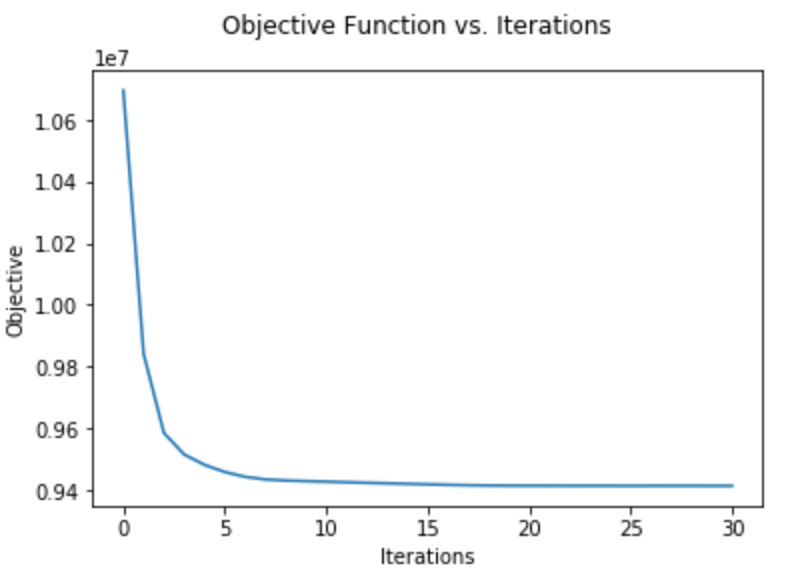
\includegraphics{2_1.png}
\end{center}

Indeed, this function never increases.

\item

Below is a graph of the final Kmeans objective versus the number of cluster means (K) used in the algorithm. I ran $10$ random restarts at each value of K and calculated the mean objective and the variance of the objective. For readability purposes, I sclaed these variances by a factor of 0.0008 to make their corresponding errorbars visible given the scale of the plot. (I played around with this number until I found one that made the graph the most readable).

\begin{center}
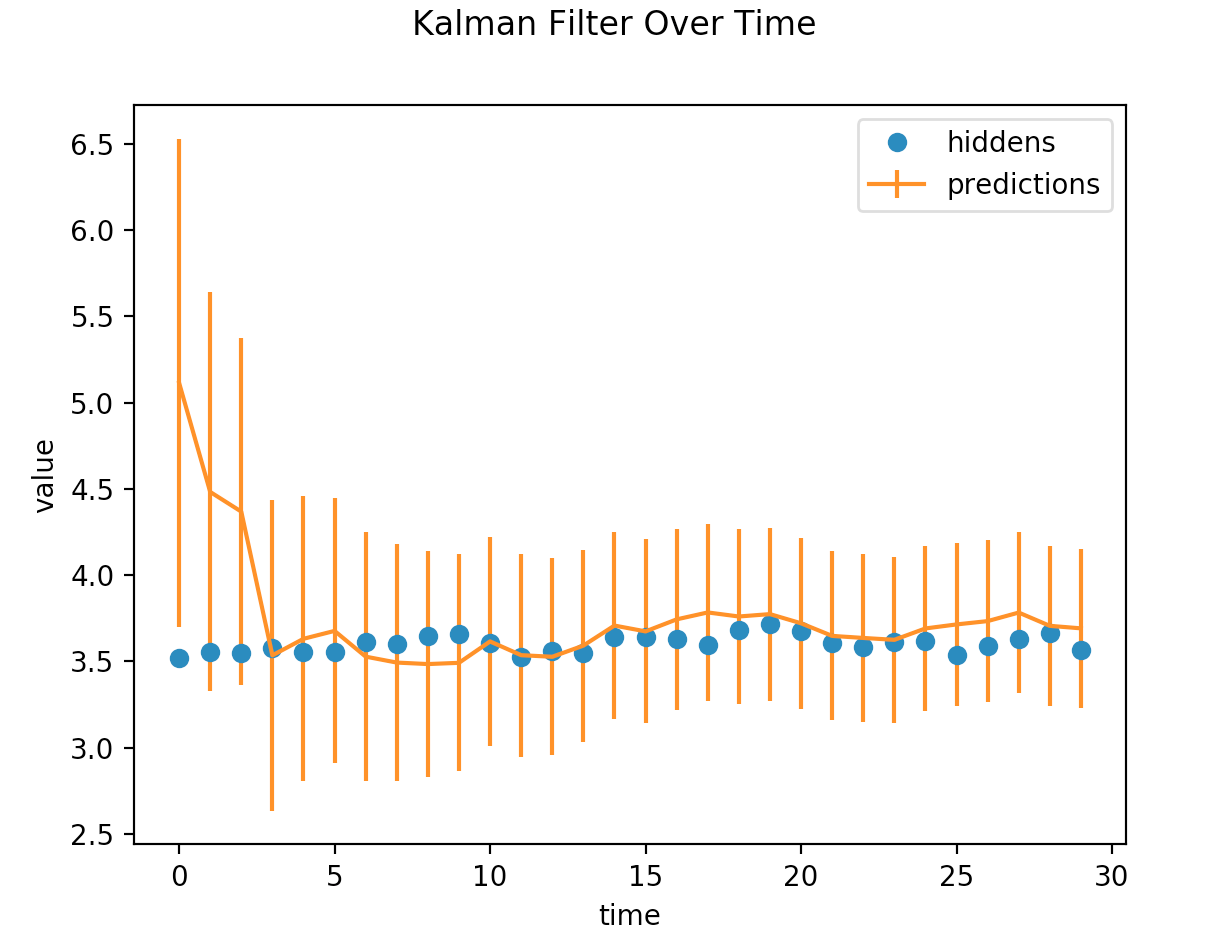
\includegraphics{2_2.png}
\end{center}

As can be seen, the objective decreases as K increases. This makes sense because with more cluster means the algorithm can better minimize the distance between each point and its cluster mean. 

The variances of the final objective appear to be relatively constant as a function of K, although they appear to have some random fluctuations (I recreated this graph many times and found that indeed the variance for a given K fluctuates between restarts). Perhaps the variance may be increasing for higher K values, but this trend appears minimal if it does exist.

\item

Below are the mean images from 4 restarts of the Kmeans algorithm with $K=10$. 

\begin{center}
\begin{tabular}{ l c r }
  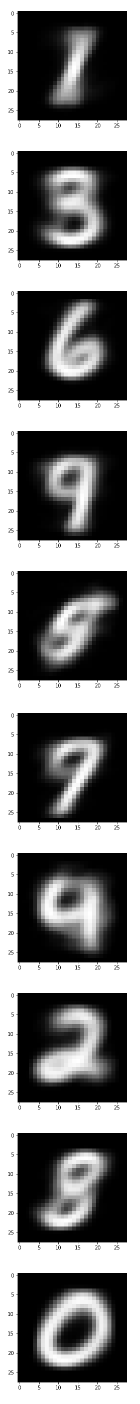
\includegraphics[scale=0.4]{2_31.png} & 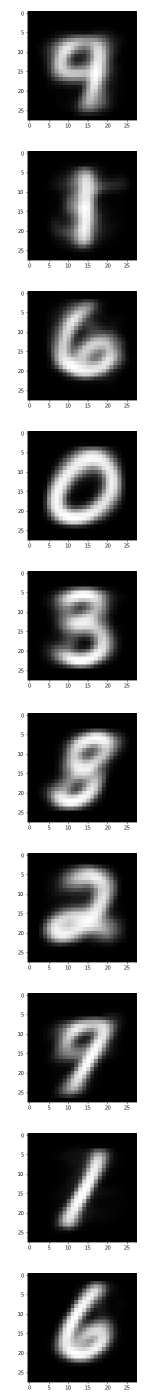
\includegraphics[scale=0.4]{2_32.png} \\
  Restart 1 & Restart 2 \\
   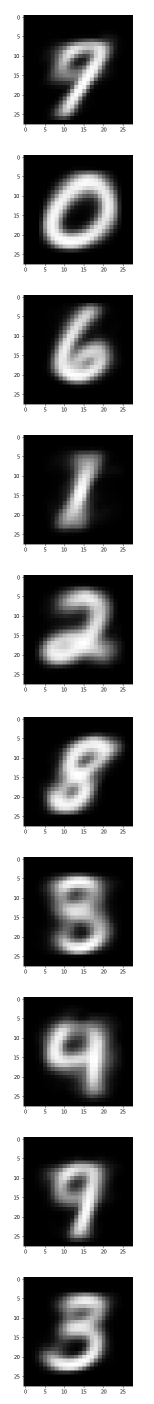
\includegraphics[scale=0.4]{2_33.png} & 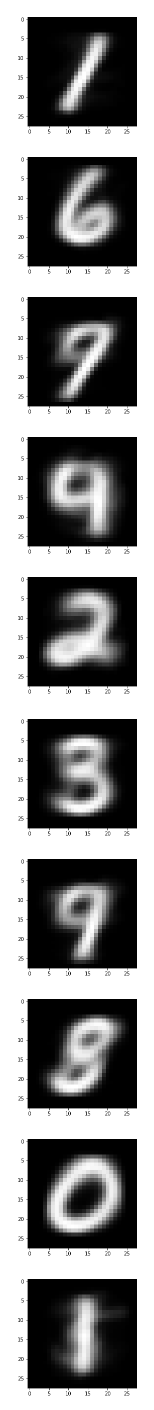
\includegraphics[scale=0.4]{2_34.png} \\
   Restart 3 & Restart 4 \\
\end{tabular}
\end{center}

These all resemble digits! Although in two of the restarts there appear to be two variants of 1's.

\item 

Below are the mean images from 4 restarts of the Kmeans algorithm with $K=10$ after standardizing. 

\begin{center}
\begin{tabular}{ l c r }
  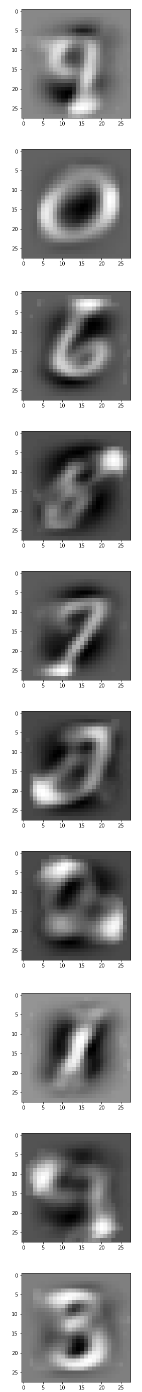
\includegraphics[scale=0.4]{2_41.png} & 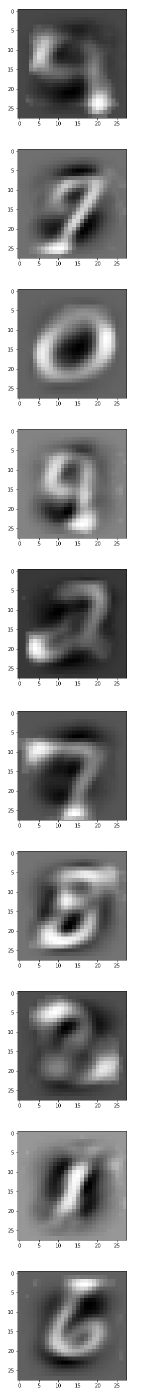
\includegraphics[scale=0.4]{2_42.png} \\
  Restart 1 & Restart 2 \\
   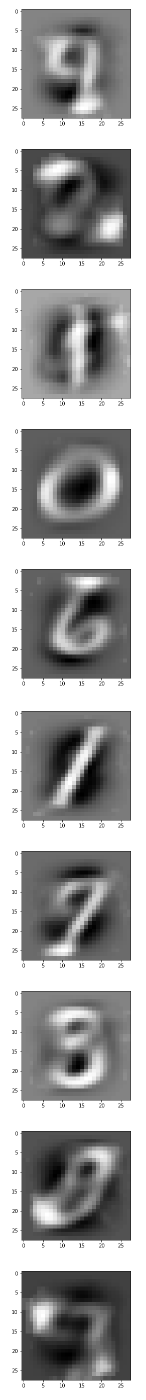
\includegraphics[scale=0.4]{2_43.png} & 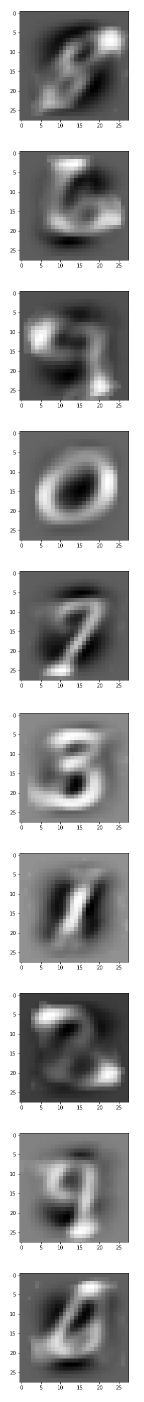
\includegraphics[scale=0.4]{2_44.png} \\
   Restart 3 & Restart 4 \\
\end{tabular}
\end{center}

These also resemble digits, as in the previous part, but they are more blurry and less easily identifiable. This is in part due to the fact that subtracting the mean made some pixels negative, and python makes the most negative pixel black and rescales all other pixels accordingly. Because of this, the backgrounds are now grey (although they had mean 0 so they should have been left unchanged). Anyways, this is to say that this adds to the indistinctness of the digits. But, even with this, the images seem to resemble digits less and are more often mixtures of multiple digits than when we did not standardize the data.

\end{itemize}

\newpage
%%%%%%%%%%%%%%%%%%%%%%%%%%%%%%%%%%%%%%%%%%%%%
% Problem 3
%%%%%%%%%%%%%%%%%%%%%%%%%%%%%%%%%%%%%%%%%%%%%
\begin{problem}[Ethics Assignment, 10pts]
\textbf{Our class activity:}

\begin{quote}
Hiring at Forever 28. Forever 28 has hired a new computer science team
to design an algorithm to predict the success of various job
applicants to sales positions at Forever 28. As you go through the
data and design the algorithm, you notice that African-American sales
representatives have significantly fewer average sales than white
sales representatives, and the most profit comes from interactions
between white female sales representatives and white male customers.
The algorithm's output recommends hiring far fewer African-Americans
than white applicants, even after the percentage of applications from
people of various races are adjusted for, and having those sales
representatives target white male customers.
\end{quote}

In class, we assumed that the problem was \textit{static}: given
historical data, such as data about sales performance, who should
Forever 28 hire right now?  In this follow-up assignment, think
about consumer behavior and firm hiring practice dynamically. Looking
at features of the labor market dynamically allows you different
degrees of freedom in your model. For example, in class, you probably
took consumer preference about the race of their sales representative
as given. What would happen if you assumed that consumer preference
could vary over time (say, on the basis of changing racial
demographics in the sales force)?

\textbf{Your new case:}
\begin{quote}
The US Secretary of Labor has heard about your team's success with Forever 28 and comes to you with a request. The Department of Labor wants to reduce disparate impact discrimination in hiring. They want you to come up with a model of fair hiring practices in the labor market that will reduce disparate impact while also producing good outcomes for companies. 
\end{quote}

Write two to three paragraphs that address the following:
\begin{itemize}
\item What is disparate impact, and how does it differ from disparate treatment?  
\item What are the relevant outcomes, for both workers and companies?  Are these outcomes measurable?  
\item What are some properties of your algorithm that might produce those socially good results?  Think about constraints that you might build in, such as the fairness constraints that we discussed in class, or how you might specify the prediction task that we are asking the machine to optimize.  [Optional] What trade-offs might your algorithm have to balance?  
\item Recommend a deployment strategy.  Are there any features of the data collection, algorithm implementation, or broader context that make you wary?  Describe how your algorithm might fit into the broader context of a company (e.g. hiring, training, marketing, sales).  
\end{itemize} 

We expect clear, concise, and thoughtful engagement with this question, which includes providing your reasoning for your answers.  In your response, depth is more important than breadth.  For example, in question 1, you could simply choose profit for the outcome that companies may be interested in; you can run with a single fairness criterion. We do \emph{not} expect you to do any outside research, though we encourage you to connect to lecture materials where relevant.

\end{problem}

\subsection*{Solution}
  
  Disparate impact occurs when the consequences of classifications or decision making disproportionately affects a certain group without intent to affect this group. In contrast, disparate treatment involves classifying someone in an impermissible way and the intent to discriminate. Disparate impact can occur when policies, guidelines, algorithms, etc. have a disproportionate impact on a group with protected attributes, like age, disability, race, gender, religion, sex, and other characteristics.

In this scenario, we must consider both the workers and the companies' relevant outcomes. For simplicity, I will assume companies care only about two things: maximizing profit, meaning their relevant outcome would be a worker's effect on profit, and their public image. The first outcome, profitability of an employee, can only be measured well sometimes. For instance, the sales of a sales person, the P/L of a stock trader, etc., can be measured clearly but it is hard to measure profitability for other positions (e.g. what's the profitability of a secretary?). The second outcome, is less quantifiable, but a company could measure its public image by taking surveys of consumers. For workers, the relevant outcomes I will consider are whether that worker was hired and the enjoyment/fulfillment of that worker in their position. The first outcome is easily measurable (it's yes or no) while the second outcome, worker fulfillment, is hard to measure but could be proxied by how long the employee stays with the company or possibly measured accurately with anonymous surveys.

In order to create this algorithm in a way that will reduce disparate impact, we will need to create a fairness criterion. For this problem, I will make this criterion that the demographics of the employees of the company must match, within some tolerance level, the demographics of the local population within which the company is operating for all protected characteristics, for all levels of employment at the company, and for all areas the company operates in. For example, considering the upper management level of employment, we would create sum cost $ \sum_{i=1}^n (g_i- p_i)^2 $ where $g_i$ is the percentage of a subset of a protected characteristic in the local area the company is operating in and $p_i$ is the percentage of upper management which is in this subset, and we sum across subsets. For instance, we could be considering gender, and we would take the difference between overall percentage of women in the area the company is operating in and the overall percentage of women in upper management of the company and similarly for men. This would also be done for every other protected characteristic (race, religion, etc). Then, for every level of the company, we would ensure that this cost is below some predetermined threshold, and we would do this in every area the city operates in (e.g. city, state, country depending on the size of the company). Achieving this seems that it would ensure fairness (in the way we have defined it) but this may come at the cost of profitability or other relevant outcomes earlier defined. Allowing for a higher threshold at each level of the company would allow for the other outcomes to be more easily achieved but will cause the fairness criterion to be fulfilled less. 

Another way we could approach this problem is trying to achieve a well-calibrated system. We could give some test of abilities needed for a job (e.g. for a sales position, how much can you sell on a first trial day?). Then, given this variable, R, we would say that $P(Y=1|R = r, A = 1) = P(Y=0|R = r,A = 0) $ where Y is the hiring outcome and A is a protected attribute. So, this means that if two candidate perform equally well on the test, they should have the same probability of being hired regardless of their protected characteristic. Accomplishing this may result in a conflict with the fairness criterion already established. If that's the case, I would think that perhaps the test has some intrinsic bias/discrimination built into it, and the test should be examined and potentially modified or scored differently. This could be a hard thing to fix, and I am wary of it.

To deploy these guidelines, the hiring decisions and current employment at the company can be analyzed to ensure that the demographics at each level of the company matches local demographics and the hiring process is well-calibrated. However, it's possible that not all demographics are applying to every position, so this could also result in failure to meet the guidelines. If this is the case, the company could consider encouragement initiatives to try and get applicants of underrepresented demographics to apply. However, this could be argued by others as discrimination against the groups whom are not being encouraged to apply, so this must be handled carefully. In the case where all demographics are applying to each position but the two conditions established above are still not being achieved, the hiring test may need to be modified or the process to determine whether someone is hired may need to be modified to adjust for protected demographics (i.e. some form of affirmative action). This will cause the fairness criterions to be achieved, but it could also help with other outcomes like public image and even profitability because a diverse workforce can lead to positive externalities such as more creativity.

Ultimately, it is clear this is a very difficult problem, but I hope my discussion demonstrates that I have thought about the task considerably.

\newpage

\begin{itemize}
    \item Name: Zachary Dietz
    \item Email: zachdietz1@gmail.com
    \item Collaborators: Theo Walker
    \item Approximately how long did this homework take you to complete (in hours):   10
\end{itemize}

\end{document}




